\section{间隔与支持向量}
给定训练样本集$D=\{(x_1,y_1),\dots,(x_m,y_m)\},y_i\in \{-1,+1\}$,分类学习最基本的想法是基于训练集D在样本空间中找到一个划分超平面,将不同类别的样本分开。如图$\ref{fig:1}$
\begin{figure}
	\centering
	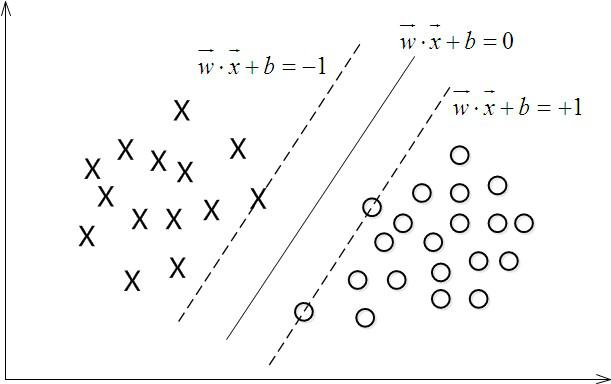
\includegraphics[width=0.7\linewidth]{chapter/统计机器学习/支持向量机/1}
	\caption{}
	\label{fig:1}
\end{figure}

样本空间中任意点$\boldsymbol{x}$到超平面$(\boldsymbol{w},b)$的距离可写为
$$\gamma = \frac{y(w^T x + b)}{\lVert w\rVert} = \frac{yf(x)}{\lVert w \rVert}$$

注:$yf(x)$相当于$\lvert f(x) \rvert$。

假设超平面$(\boldsymbol{w},b)$能将训练样本正确分类,即对于$(x_i,y_i)\in D$,若$y_i=+1,$则有$\boldsymbol{w}^Tx_i+b>0$;若$y_i=-1$,则有$\boldsymbol{w}^Tx_i+b<0$。令
\begin{equation}
\label{eq:1}
\begin{cases} 
\boldsymbol{w}^Tx_i+b\geq +1,\quad y_i=+1;\\
\boldsymbol{w}^Tx_i+b\leq -1,\quad y_i=-1.
\end{cases}
\end{equation}

距离超平面最近的这几个训练样本点使式$\ref{eq:1}$的等号成立,它们被称为“\textbf{支持向量}(support vector)”,两个异类支持向量到超平面的距离之和为
\begin{equation}
	\label{eq:2}
	\gamma = \frac{2}{\lVert w \rVert},
\end{equation}
它被称为“\textbf{间隔}”(margin)。

欲找到具有“最大间隔”的划分超平面,也就是要找到能满足式$\ref{eq:1}$中约束的参数$\boldsymbol{w}$和$b$,使得$\gamma$最大,即
\begin{equation}
	\label{eq:3}
	\begin{aligned}
	min \quad &\frac{1}{2}\lVert w \rVert^2, \\
	s.t. \quad & y_i (w^Tx _i + b) \geq 1, \quad i = 1,\dots, m.
	\end{aligned}
\end{equation}
这就是支持向量机的基本型。

